\documentclass{article}

\usepackage{tikz}
\usetikzlibrary{arrows, decorations.pathmorphing, backgrounds, positioning, fit, 
	petri}
\begin{document}

% path usage: we're moving to given coordinate, writing empty text (inside
% curly brackets), drawing shape around text and then moving forward according
% to path
\begin{tikzpicture}
  \path ( 0,2) node [shape = circle,draw]    {}
        ( 0,1) node [shape = circle,draw]    {}
        ( 0,0) node [shape = circle,draw]    {}
        ( 1,1) node [shape = rectangle,draw] {}
        (-1,1) node [shape = rectangle,draw] {};
\end{tikzpicture}

\vspace{1cm}

% something nearly the same happening here, although the syntax is simpler
% the trick here is that \node command is an abbreviation for \path node, so 
% implicitly we have here an amount of nodes on paths
\begin{tikzpicture}
  \node at ( 0,2) [circle, draw] {};
  \node at ( 0,1) [circle, draw] {};
  \node at ( 0,0) [circle, draw] {};
  \node at ( 1,1) [rectangle, draw] {};
  \node at (-1,1) [rectangle, draw] {};
\end{tikzpicture}

\vspace{1cm}

% adding some style to elements, defining some "classes"
% adding names to nodes inside round brackets
% use relative positioning instead of absolute
% adding another node with the capacity above it
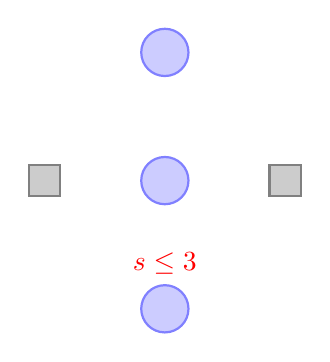
\begin{tikzpicture}
  [place/.style={circle,draw=blue!50,fill=blue!20,thick,
   inner sep = 0pt, minimum size=6mm},
   transition/.style={rectangle,thick,draw=black!50,fill=black!20,
                      inner sep=0pt,minimum size=4mm}]
   \node[place]      (waiting)                                     {};
   \node[place]      (critical)       [below=of waiting]           {};
   \node[place]      (semaphore)      [below=of critical,
    								   label={[red]above:$s\le3$}] {};
   \node[transition] (leave critical) [right=of critical]          {};
   \node[transition] (enter critical) [left=of critical]           {};
\end{tikzpicture}

\vspace{1cm}

% creating style entities outside of tikzpicture
\tikzstyle{place} = [circle,draw=blue!50,fill=blue!20,thick,inner sep=0pt,
					 minimum size=6mm]
\tikzstyle{transition} = [rectangle,thick,draw=black!50,fill=black!20,
						  inner sep=0pt,minimum size=4mm]

\tikzstyle{pre} = [<-,shorten <= 1pt, >=stealth',semithick]
\tikzstyle{post} = [->,shorten >= 1pt, >=stealth',semithick]

% connecting nodes
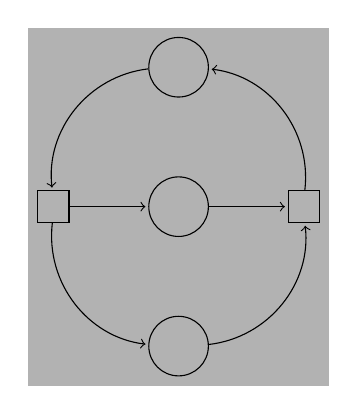
\begin{tikzpicture}
  [bend angle = 45]
  
  \node[place]      (waiting)                            {};
  \node[place]      (critical)       [below=of waiting]  {};
  \node[place]      (semaphore)      [below=of critical] {};

  \node[transition] (leave critical) [right=of critical] {}
  	edge [pre]             (critical)
  	edge [post,bend right] (waiting)
  	edge [pre, bend left]  (semaphore);

  \node[transition] (enter critical) [left=of critical]  {}
  	edge [post]             (critical)
  	edge [pre, bend left]   (waiting)
  	edge [post, bend right] (semaphore);
  
  \begin{scope}[on background layer]
    \node [fill=black!30,fit=(waiting) (critical) (semaphore) 
      (leave critical) (enter critical)] {};
  \end{scope}
\end{tikzpicture}
\end{document}